\documentclass{beamer}
\usetheme{Berlin}
\beamertemplatenavigationsymbolsempty
\usepackage[utf8]{inputenc}
\usepackage[T1]{fontenc}
\usepackage{polski}
\usepackage{wrapfig}
\usepackage{graphicx}
\usepackage{ragged2e}
\usepackage{textcomp}
\usepackage{gensymb}
\usepackage{multicol}
\usepackage{caption}
\usepackage{subcaption}
\usepackage[absolute,overlay]{textpos}
    \setlength{\TPHorizModule}{1mm}
    \setlength{\TPVertModule}{1mm}

\graphicspath{ {Images/} } %%domyslna sciezka dla obrazow

\title{Komputerowe rozpoznawanie odcisków palców}
\subtitle{Zastosowanie informatyki w medycynie}

\author{Bednarczyk Waldemar, Krymchak Veronika, Rodziewicz~Bartosz}

\institute{Politechnika Wrocławska}
\date{\today}
\usecolortheme{whale}
\usepackage{graphicx}

\begin{document}

\begin{frame}
    \titlepage
\end{frame}

\section{Wstęp}

\begin{frame}{Plan prezentacji}
    \huge
    \begin{itemize}
        \item[] \centering Historia
        \item[] Zastosowanie
        \item[] Rodzaje czytników
        \item[] Linie papilarne
        \item[] Algorytmy analizy
    \end{itemize}
\end{frame}

\begin{frame}{Wstęp}
    \justifying
    Układ linii papilarnych jest cechą charakterystyczną każdego człowieka - jest różny u każdego z Nas. Linie papilarne są cechą, której nie da się zmienić. Można się ich jedynie pozbyć celowo, np. poprzez usunięcie naskórka, wypalenie. Układ linii papilarnych opisuje się za pomocą tzw. minucji - charakterystycznych cech, takich jak początki, zakończenia, rozwidlenia, haczyki itp. Wzajemny układ minucji jednoznacznie identyfikuje daną osobę. \\
    Programy do rozpoznawania odcisków palców korzystają z rozmieszczenia minucji, porównywanie obrazów odcisków jest niemożliwe, gdyż każdy obrazy odcisku tego samego palca prawie na pewno różnią się od siebie (szumy, stosowanie innego urządzenia).
\end{frame}

\section{Historia}

\begin{frame}
    \centering
    \huge
    Historia
\end{frame}

\begin{frame}{Starożytność}
    \begin{wrapfigure}{L}{0.4\textwidth}
        \centering
        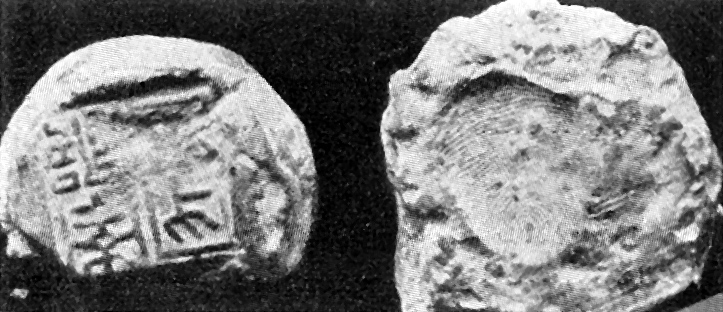
\includegraphics[width=0.4\textwidth]{History/ancient_seals.jpg}
        \caption{Chińska pieczęć}
    \end{wrapfigure}
    \justifying
    O istnieniu linii papilarnych na skórze człowieka wiedziano już w czasach starożytnych. Świadczą o tym liczne znaleziska np. petroglify, wyroby ceramiczne, rzeźby naskalne. Wiele z nich świadczy o używaniu odbitej palców jako rodzaju poświadczenia swojej tożsamości, jako podpisu, pieczęci. Np. gliniane pieczęcie z Chin (500 lat p.n.e.) posiadają z jednej strony odcisk kciuka, z drugiej strony imię.
\end{frame}

\begin{frame}{Średniowiecze}
    \begin{figure}[t]
        \centering
        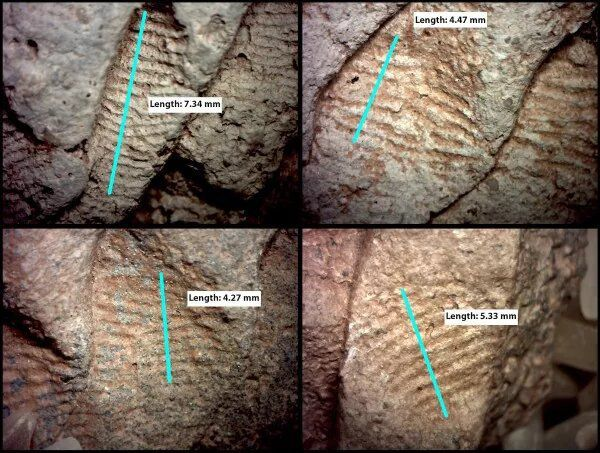
\includegraphics[width=0.5\linewidth]{History/ancient_fingerprints.jpg}
        \caption{Odciski palców na ceramicznych wazach }
    \end{figure}
\end{frame}

\begin{frame}{Johann Christoph Andreas Mayer}
\begin{columns}
    \begin{column}[T]{.6\textwidth}
    \justifying
        \begin{center}
            W 1788 w swojej książce napisał: "Chociaż układ grzbietów skóry nigdy nie jest powielany u dwóch osób, niemniej podobieństwa u niektórych osób są bliższe." Meyer jako pierwszy stwierdził unikalność linii papilarnych.
        \end{center}
    \end{column}
    \hfill
    \begin{column}[T]{.4\textwidth}
        \begin{figure}
            \centering
            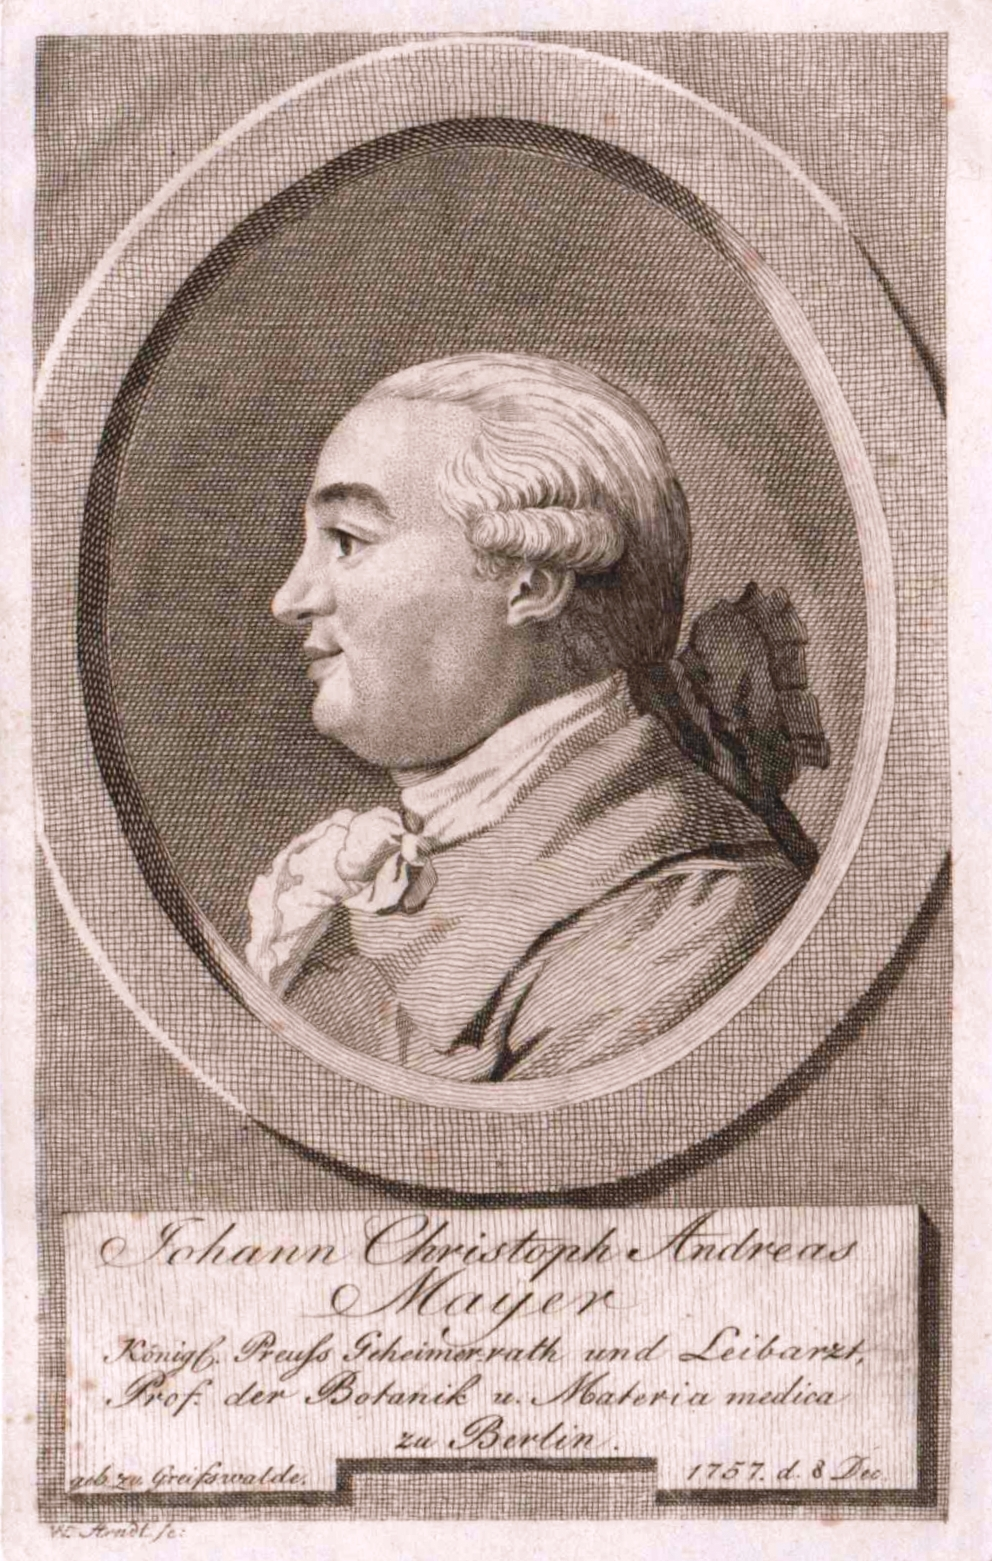
\includegraphics[width=.7\textwidth]{History/meyer.jpg}
        \end{figure}
    \end{column}
\end{columns}
\end{frame}

\begin{frame}{Sir Francis Galton}
\begin{columns}
    \begin{column}[T]{.6\textwidth}
        \begin{itemize}
            \item Pionier identyfikacji odcisków palców
            \item Udowodnił, że nie istnieją dwa takie same odciski palców
            \item Wykazał, że odcisk palca jest niezmienny przez całe życie
            \item Opracował pierwszy na świecie praktyczny system klasyfikacji oraz identyfikacji odcisków palców
        \end{itemize}
    \end{column}
    \hfill
    \begin{column}[T]{.4\textwidth}
        \begin{figure}
            \centering
            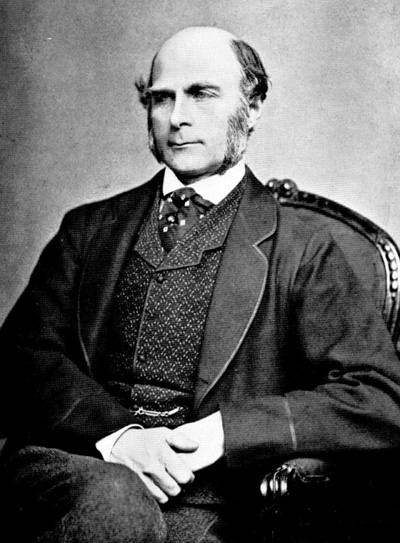
\includegraphics[width=0.7\textwidth]{History/Francis_Galton_1850s.jpg}
        \end{figure}
    \end{column}
\end{columns}
\end{frame}

\begin{frame}{Pierwsza kartoteka}
    \begin{wrapfigure}{L}{0.2\textwidth}
        \centering
        
\includegraphics[width=0.2\textwidth]{History/argentina_flag.png}
    \end{wrapfigure}
    \justifying
    W 1896 roku Argentyna została państwem, w którym po raz pierwszy odciski palców stały się podstawą policyjnej służby śledczej, pomimo tego, że zaledwie 3 lata wcześniej dyrekcja policji zakazała pracy nad daktyloskopią.

    \begin{wrapfigure}{R}{0.2\textwidth}
        \centering
        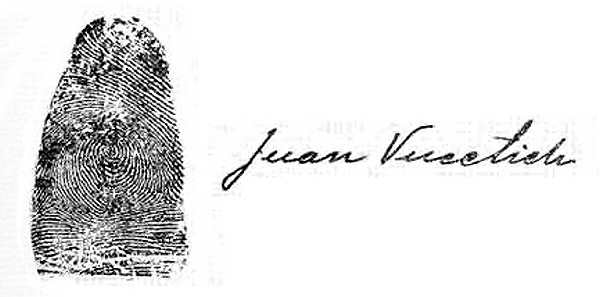
\includegraphics[width=0.2\textwidth]{History/juan_fingerprint.jpg}
    \end{wrapfigure}
    Pracownik Argentyńskiej policji, Juan Vucetich, stworzył pierwszą kartotekę z odciskami palców bazując na cechach wyodrębnionych przez Francisa Galtona.
\end{frame}

\begin{frame}{Teraźniejszość - bazy danych}
    \begin{itemize}
        \item Odciski palców 120 milionów osób
        \item 300 tysięcy wyszukiwań dziennie
    \end{itemize}
    \centering
    
\includegraphics[width=0.4\textwidth]{History/homeland-security.jpg}
\end{frame}

\section{Zastosowanie}

\begin{frame}
    \centering
    \huge
    Zastosowanie
\end{frame}

\begin{frame}{Identyfikacja / uwierzytelnianie}
    \centering
    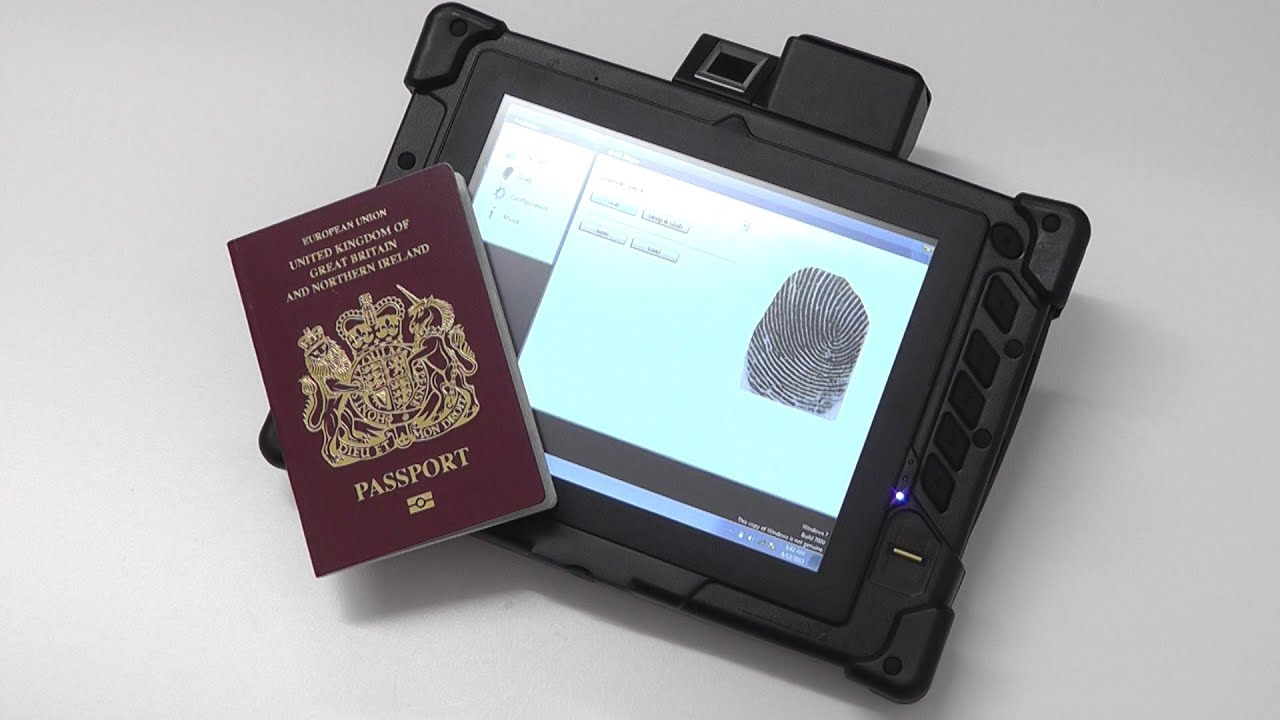
\includegraphics[width=0.8\textwidth]{History/passport_fingerprint.jpg}
\end{frame}

\begin{frame}{Kryminalistyka}
    \centering
    \includegraphics[width=0.8\textwidth]{History/Fingerprint-Criminal-Law.jpg}
\end{frame}

\begin{frame}{Systemy bezpieczeństwa}
    \centering
    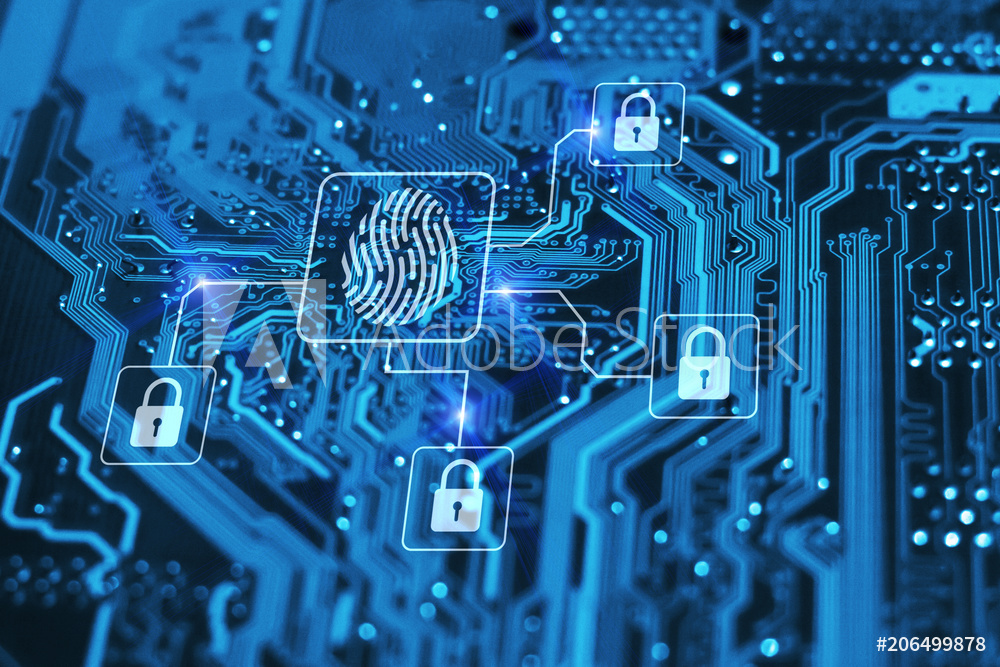
\includegraphics[width=0.6\textwidth]{History/authorization.jpg}
    \begin{itemize}
        \centering
        \item{Odpowiedź w czasie rzeczywistym}
        \item{Przeszukiwanie bazy danych}
    \end{itemize}
\end{frame}

\section{Rodzaje czytników}

\begin{frame}
    \centering
    \huge
    Rodzaje czytników
\end{frame}

\begin{frame}{Czytniki optyczne}
    \begin{itemize}
        \item najstarsze
        \item wykonują zdjęcie przyłożonego odciska palca
        \item wykorzystują do działania źródło światła, pryzmat oraz matrycę CCD
        \item łatwe do oszukania za pomocą dobrej jakości wydruku linii papilarnych
    \end{itemize}
    \smallskip
    \begin{figure}
        \centering
        \begin{subfigure}{.49\textwidth}
            \centering
            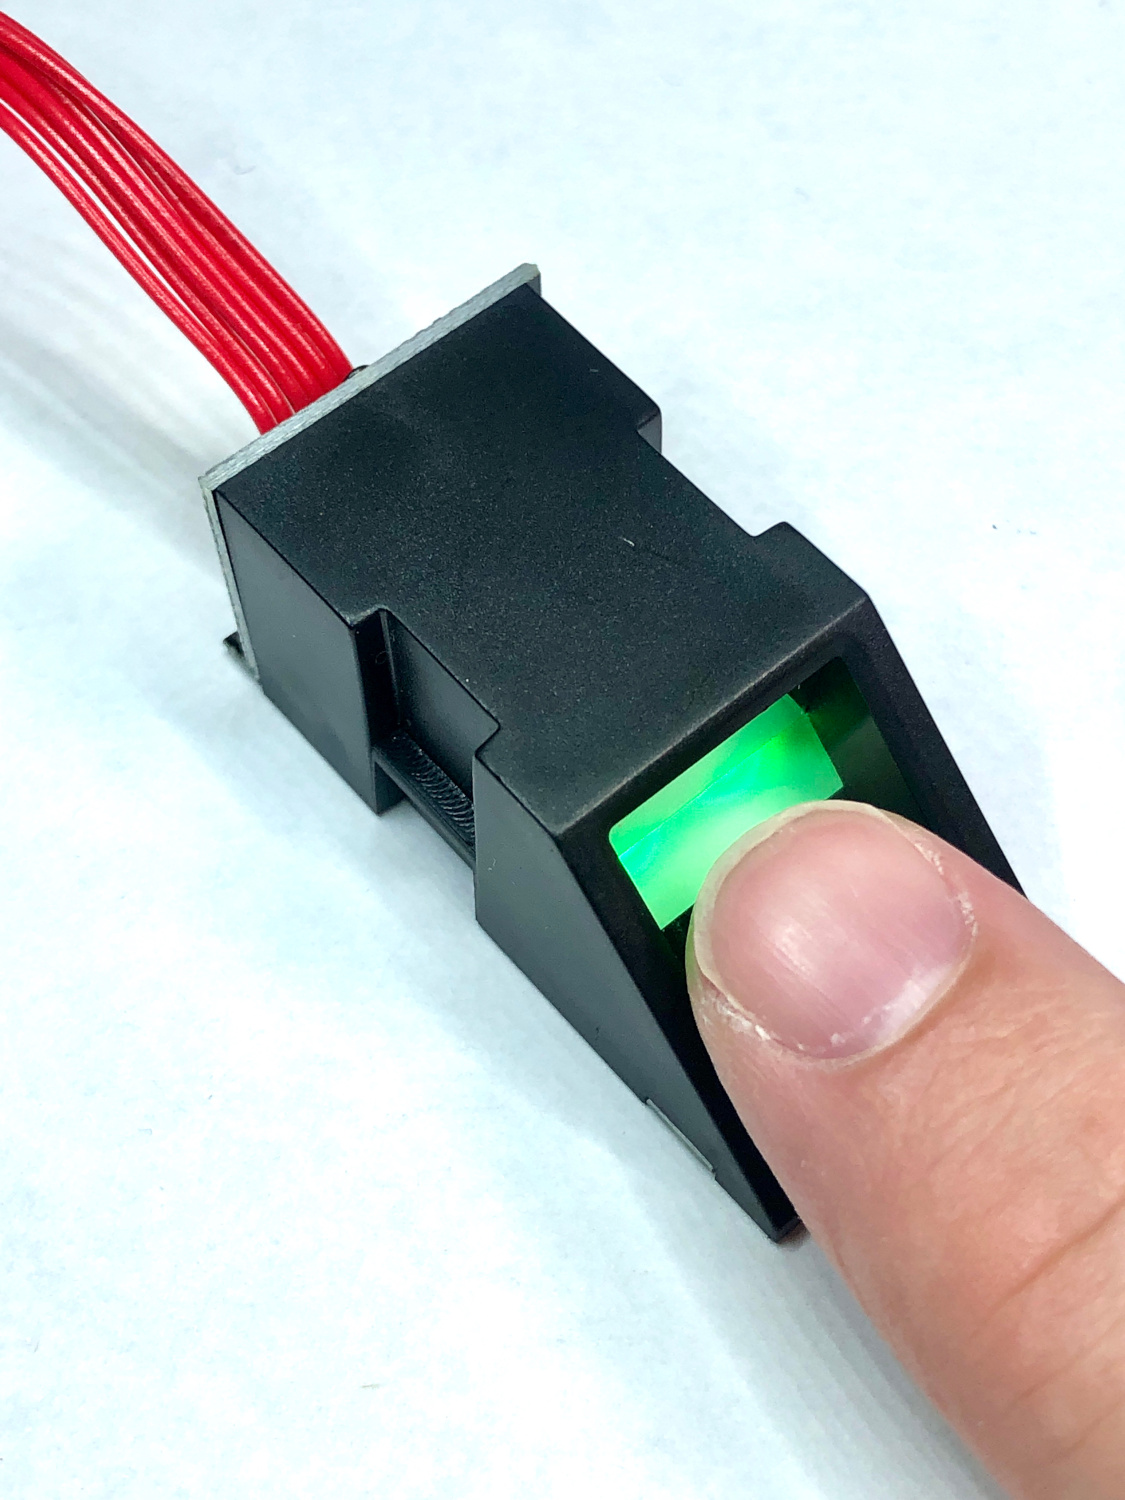
\includegraphics[width=0.3\linewidth]{types/fingerprint_as608_finger.jpg}
        \end{subfigure}
        \begin{subfigure}{.49\textwidth}
            \centering
            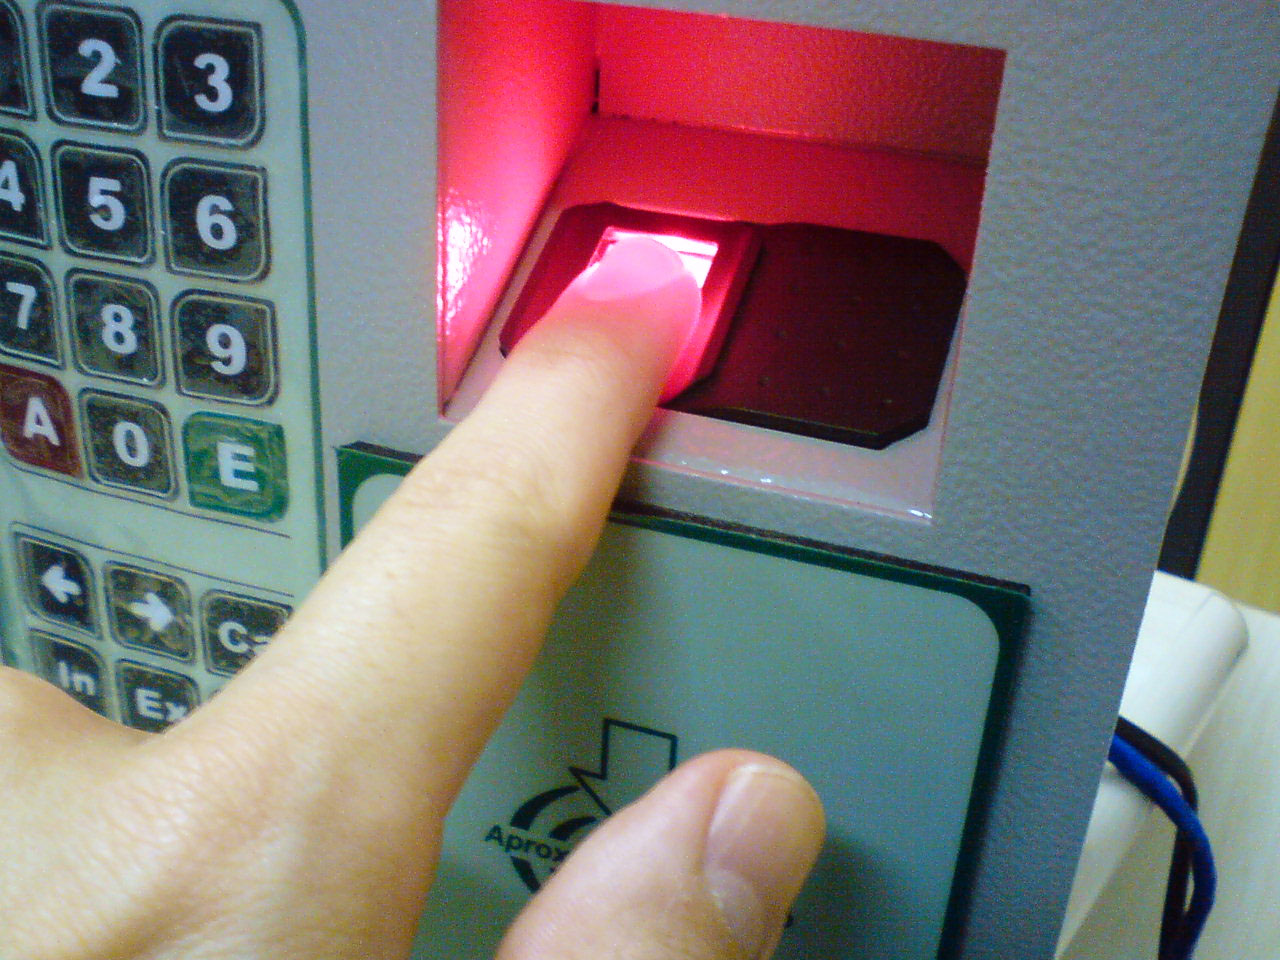
\includegraphics[width=0.5\linewidth]{types/Fingerprint_scanner_identification.jpg}
        \end{subfigure}
        \caption{Dwa przykładowe czytniki optyczne}
    \end{figure}
\end{frame}

\begin{frame}
    \begin{figure}[t]
        \centering
        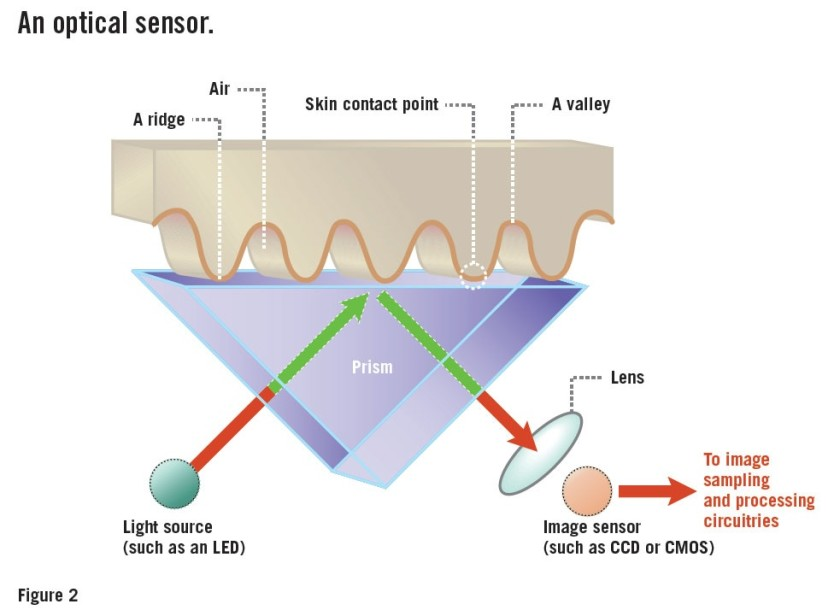
\includegraphics[width=0.85\linewidth]{types/Optical-fingerprint-scanner-840x610.jpg}
        \caption{Zasada działania czytnika optycznego}
    \end{figure}
\end{frame}

\begin{frame}
    \begin{figure}[t]
        \centering
        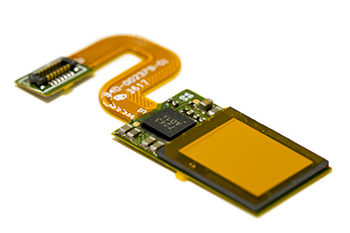
\includegraphics[width=0.85\linewidth]{types/Synaptics_Clear_ID_optical_fingerprint_sensor.png}
        \caption{Zminiaturyzowany czytnik optyczny}
    \end{figure}
\end{frame}

\begin{frame}{Czytniki pojemnościowe}
    \begin{itemize}
        \item najpopularniejsze (przynajmniej w zastosowaniach konsumenckich)
        \item wykorzystują w działaniu fakt, że skóra ludzka przewodzi prąd
        \item powierzchnia zbudowana jest z matrycy kondensatorów wykrywającej zmiany pojemności ich pojemności elektrycznej
        \item zastępują czytniki optyczne
    \end{itemize}
    \medskip
    \begin{figure}
        \centering
        \begin{subfigure}{.49\textwidth}
            \centering
            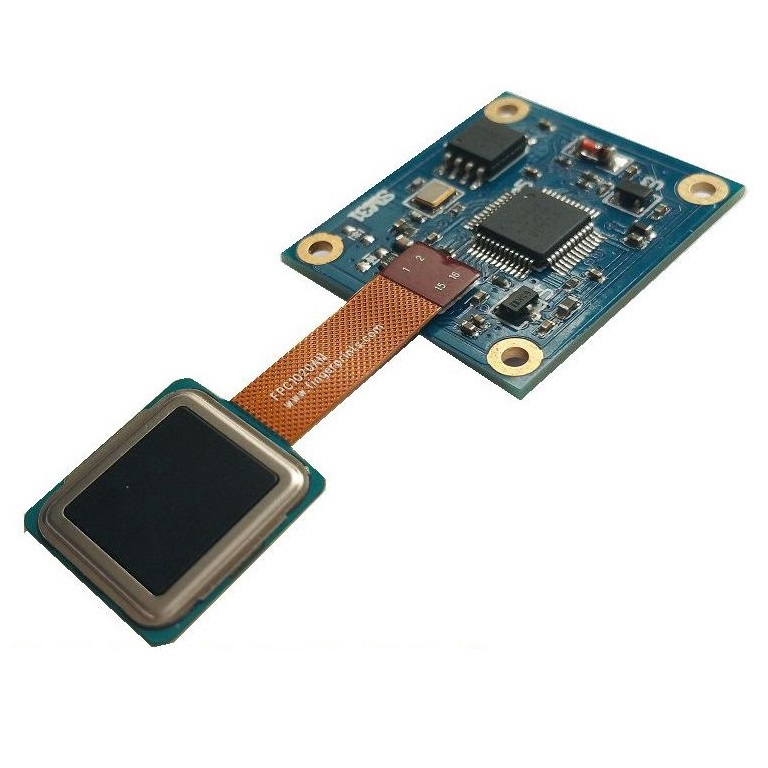
\includegraphics[width=0.5\linewidth]{types/CAMA-AFM31-USB-Capacitive-Fingerprint-Module-with-FPC1020-Fingerprint-Sensor-Arduino-01.jpg}
        \end{subfigure}
        \begin{subfigure}{.49\textwidth}
            \centering
            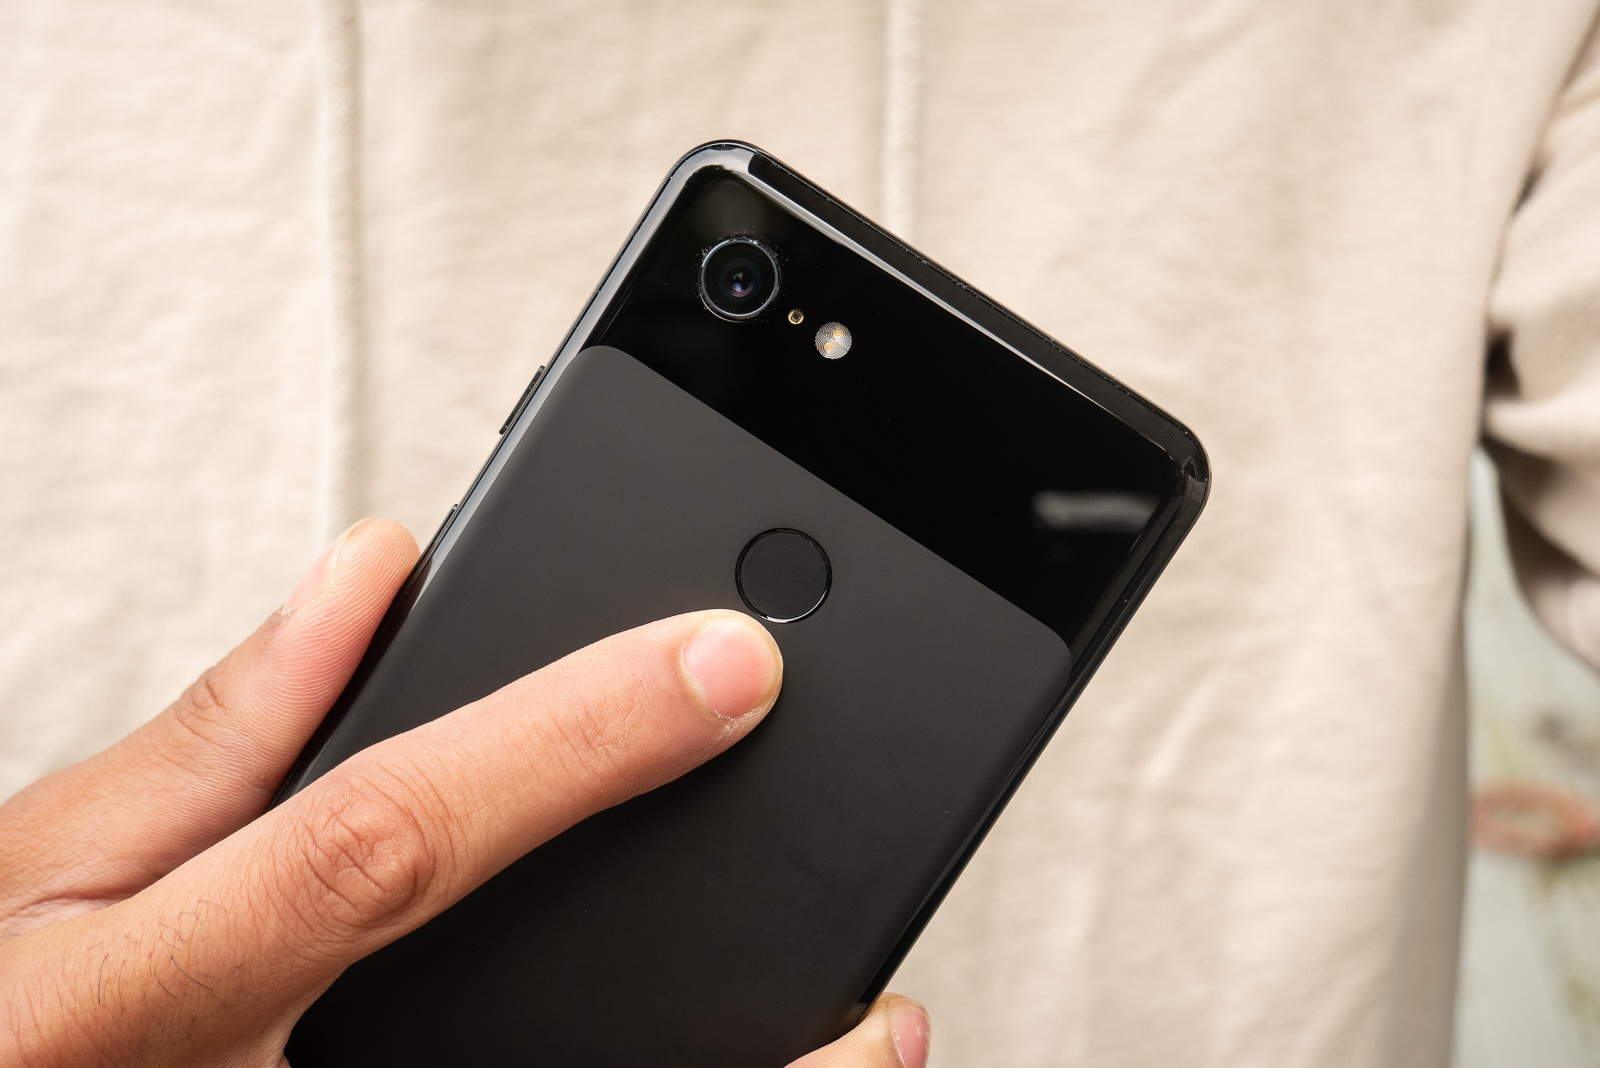
\includegraphics[width=0.7\linewidth]{types/Google-Pixel-3-and-Pixel-3-XL-users-are-now-facing-fingerprint-gesture-inconsistencies.jpg}
        \end{subfigure}
        \caption{Dwa przykładowe czytniki pojemnościowe}
    \end{figure}
\end{frame}

\begin{frame}{Czytniki ultradźwiękowe}
    \begin{itemize}
        \item działają wykorzystując fale dźwiękowe niesłyszalne przez człowieka i polegając na zjawisku dyfrakcji
        \item potrafią wytworzyć model 3D palca
        \item najbezpieczniejsze i najcięższe do oszukania
        \item czytnik może znajdować się pod warstwą szkła, metalu bądź plastiku
    \end{itemize}
    \begin{figure}
        \centering
        \begin{subfigure}{.49\textwidth}
            \centering
            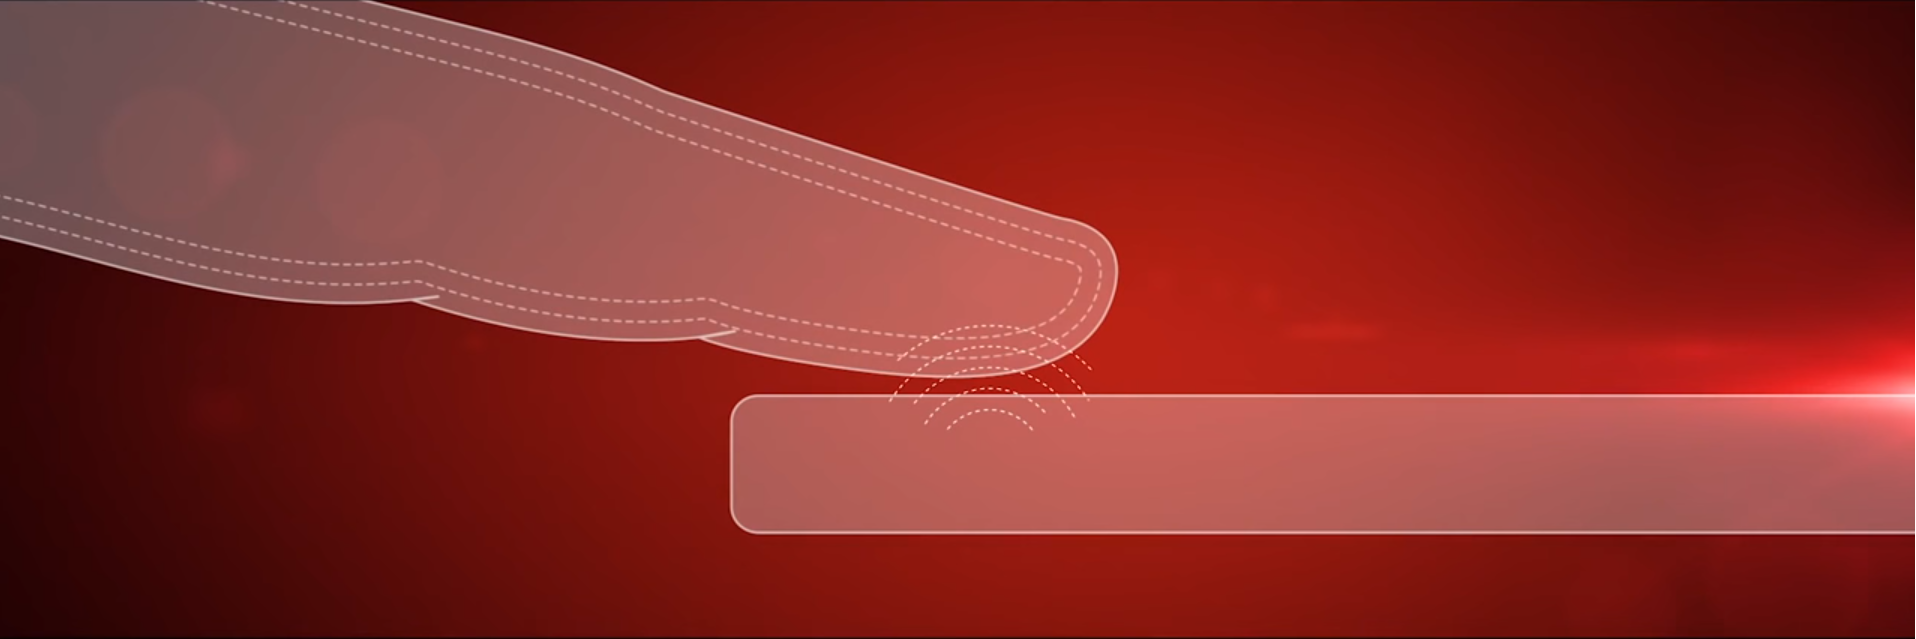
\includegraphics[width=\linewidth]{types/ultrasonic.png}
        \end{subfigure}
        \begin{subfigure}{.49\textwidth}
            \centering
            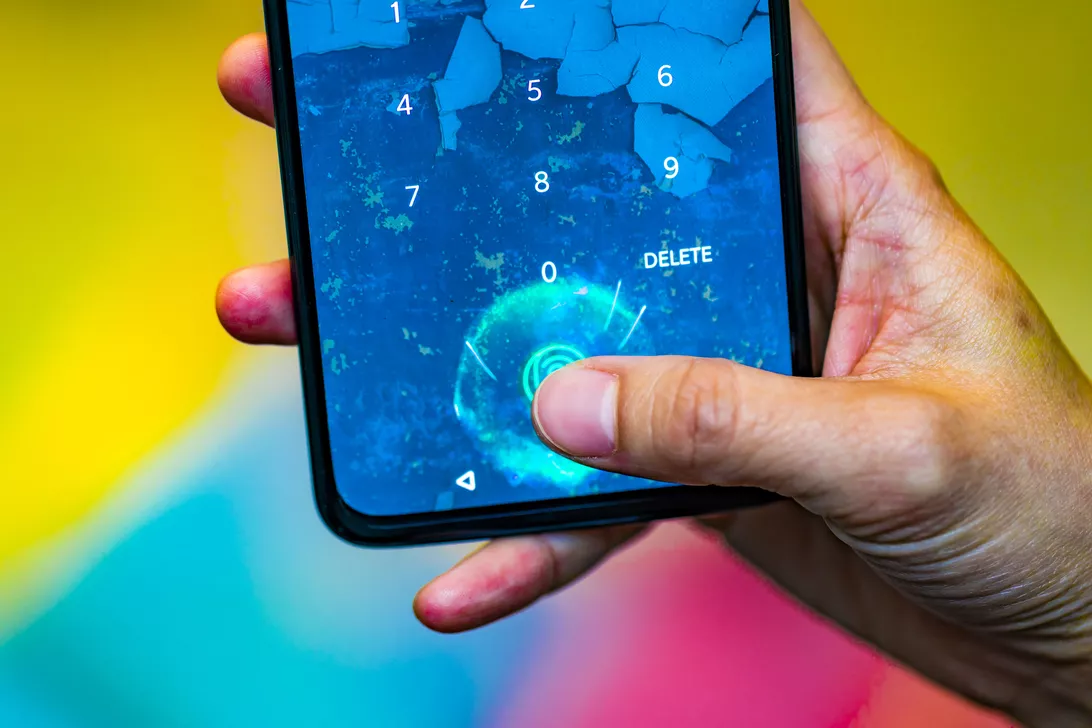
\includegraphics[width=0.7\linewidth]{types/oneplus-6t-3435.png}
        \end{subfigure}
    \end{figure}
\end{frame}

\begin{frame}{Inne rodzaje czytników}
    \begin{itemize}
        \item termiczne
        \item nacisku
        \item radiowe
    \end{itemize}
    \bigskip
    \begin{figure}
        \centering
        \begin{subfigure}{.49\textwidth}
            \centering
            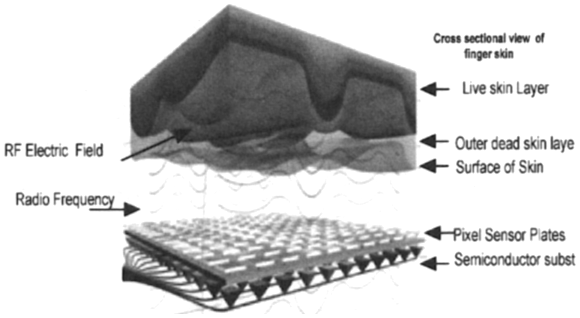
\includegraphics[width=0.9\linewidth]{types/Radio-Frequency-RF-based-Fingerprint-Sensor-14.png}
        \end{subfigure}
        \begin{subfigure}{.49\textwidth}
            \centering
            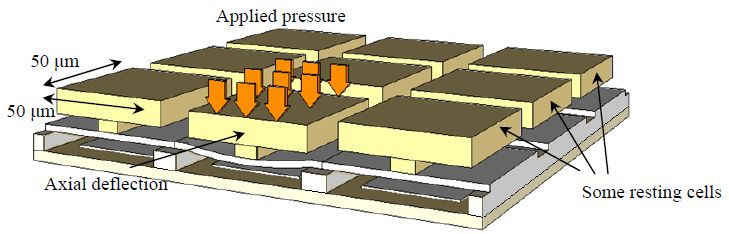
\includegraphics[width=0.9\linewidth]{types/IMEN_MEMScapacitive.jpg}
        \end{subfigure}
    \end{figure}
\end{frame}

\begin{frame}{Podział czytników ze względu na budowę}
    \begin{itemize}
        \item statyczne
            \begin{itemize}
            	\item bardziej dokładne
            	\item aktualnie częściej spotykane
        	\end{itemize}
        \item przesuwne
            \begin{itemize}
            	\item tańsze
            	\item zajmują mniej miejsca
        	\end{itemize}
    \end{itemize}
    \bigskip
    \begin{figure}
        \centering
        \begin{subfigure}{.49\textwidth}
            \centering
            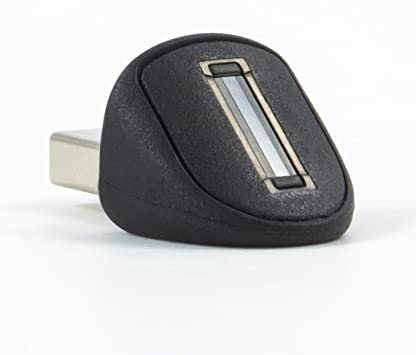
\includegraphics[width=0.9\linewidth]{types/61yjiAyKfnL._AC_SY355_.jpg}
        \end{subfigure}
        \begin{subfigure}{.49\textwidth}
            \centering
            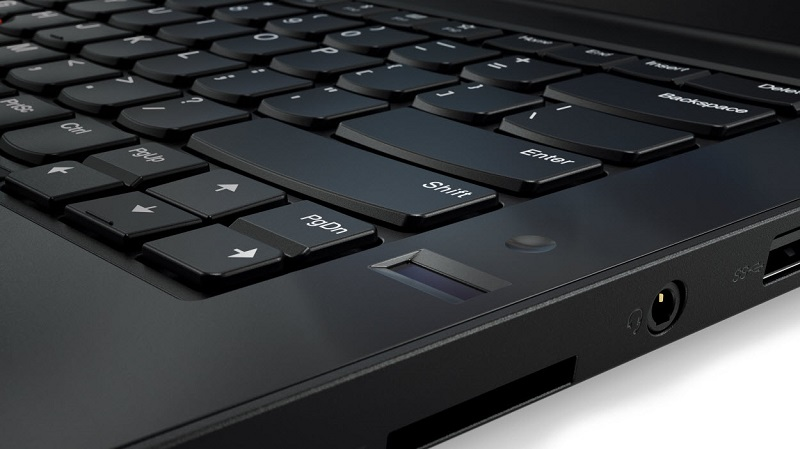
\includegraphics[width=0.8\linewidth]{types/Lenovo_ThinkPad_fingerprint_reader.jpg}
        \end{subfigure}
    \end{figure}
\end{frame}

\section{Linie papilarne}

\begin{frame}
    \centering
    \huge
    Linie papilarne
\end{frame}

\begin{frame}{Co to są linie papilarne?}
    Linie papilarne – jest to charakterystyczny układ bruzd na skórze ssaków naczelnych, w szczególności na opuszkach palców rąk, ale również na wewnętrznej powierzchni dłoni, palcach stóp i wargach.
\end{frame}

\begin{frame}{Właściwości linii papilarnych}
    \begin{itemize}
        \item{Niepowtarzalność - nie ma dwóch osób, które miałyby taki sam układ linii papilarnych.}
        \item{Niezmienność - przez całe życie układ linii papilarnych pozostaje taki sam. Linie papilarne ulegają jedynie wzrostowi. Wzór i cechy szczegółowe pozostają takie same przez całe życie aż do rozkładu gnilnego zwłok}
        \item{Niezniszczalność - linie papilarne mają zdolność regeneracji, odradzają się po wyleczeniu skaleczeń, chorób skóry lub po ustaniu przyczyn ścierania naskórka (np. wykonywanie pracy fizycznej). Jedynie uszkodzenie skóry właściwej powoduje powstanie blizny, która może się stać cechą indywidualizującą}
    \end{itemize}
\end{frame}

\begin{frame}{Grupy wzorów linij papilarnych}
    Wyróżnia się struktury, które są podstawą do budowy złożonych wzorów rozpoznawanych na opuszku palca:
    \begin{itemize}
        \item{Delta - tworzą ją dwie linie równoległe, które rozchylają się w pewnym punkcie w kształt lejka}
    \end{itemize}
    \begin{figure}[t]
        \centering
        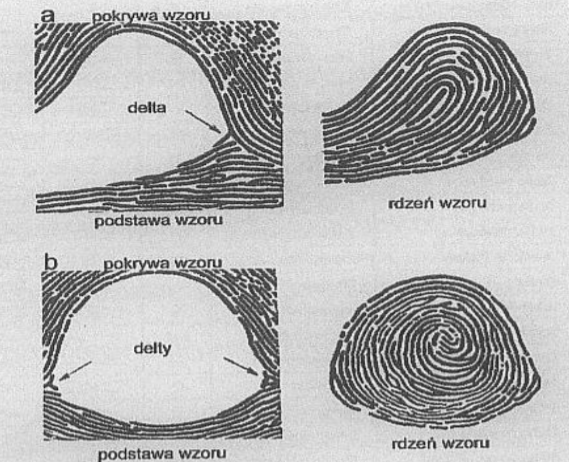
\includegraphics[width=0.4\textwidth]{fingerprints/delta.png}
    \end{figure}
\end{frame}

\begin{frame}{Grupy wzorów linij papilarnych}
    \begin{itemize}
        \item{Termin wewnętrzny - jest to punkt wyznaczony w centrum wzoru}
        \item{Termin zewnętrzny - jest to punkt wyznaczony w obrębie delty}
    \end{itemize}
    \begin{figure}[t]
        \centering
        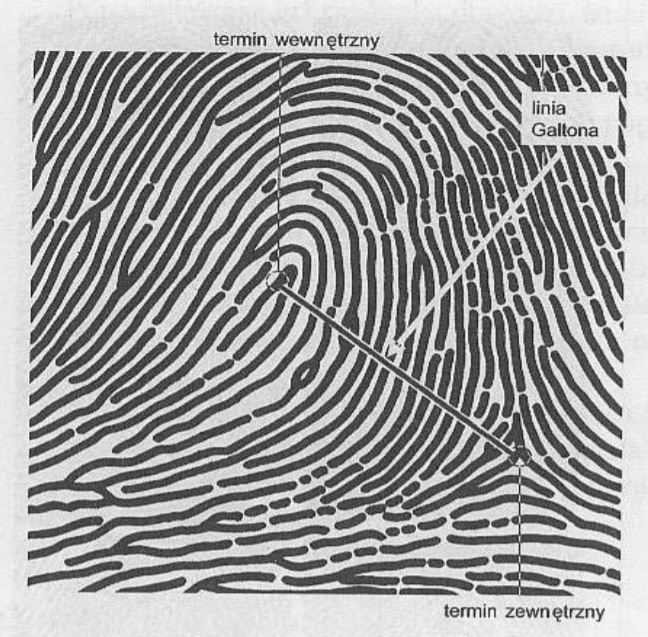
\includegraphics[width=0.35\textwidth]{fingerprints/liniaGaltona.png}
    \end{figure}
    \begin{itemize}
        \item{linia Galtona - łączy termin zewnętrzny z terminem wewnętrznym}
    \end{itemize}
\end{frame}

\begin{frame}{Grupy wzorów linij papilarnych}
    \begin{figure}[t]
        \centering
        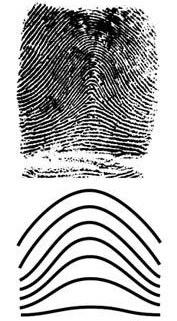
\includegraphics[width=0.2\textwidth]{fingerprints/lukowy.jpg}
    \end{figure}
    Wzory łukowe.
    Są najrzadziej spotykane (ok.6\%). Charakteryzują się brakiem delty i rdzenia
\end{frame}

\begin{frame}{Grupy wzorów linij papilarnych}
    \begin{figure}[t]
        \centering
        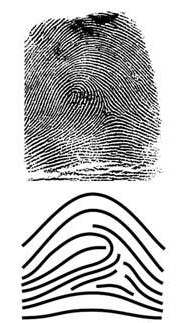
\includegraphics[width=0.2\textwidth]{fingerprints/petlicowy.jpg}
    \end{figure}
    Wzory pętlicowe.
    Występują najczęściej (64\%) Wzór taki musi posiadać: tylko jedną deltę, przynajmniej jedną pętlicę, przynajmniej jedną linię papilarną przecinającą linie Galtona.
\end{frame}

\begin{frame}{Grupy wzorów linij papilarnych}
    \begin{figure}[t]
        \centering
        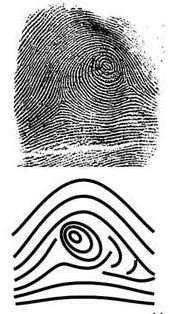
\includegraphics[width=0.2\textwidth]{fingerprints/wirowy.jpg}
    \end{figure}
    Wzory wirowe (30\%). Charakteryzują się najbardziej złożoną budową. Ich rdzeń tworzą koła elipsy, spirale, pętlice i inne wzory.
\end{frame}

\begin{frame}{Minucje}
    Są to charakterystyczne zmiany przebiegu linii papilarnych. Służą do opisu odcisków palców. Ich układ może posłużyć do jednoznacznego opisu każdego odcisku.
    Wyróżniają:
    \begin{itemize}
        \item{Początki}
        \item{Zakończenia}
        \item{Rozwidlenia}
        \item{Haczyki}
    \end{itemize}
\end{frame}

\begin{frame}{Minucje}
    \begin{columns}
        \column{0.25\textwidth}
            \begin{figure}[t]
			    \centering
                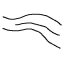
\includegraphics[width=0.4\textwidth]{fingerprints/minucje/poczatek.jpg}\\~\
                 \caption*{Początek}
            \end{figure}
           
		\column{0.25\textwidth}
		    \begin{figure}[t]
			    \centering
                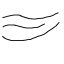
\includegraphics[width=0.4\textwidth]{fingerprints/minucje/zakonczenie.jpg}
                \caption*{Zakończenie}
            \end{figure}
        \column{0.25\textwidth}
            \begin{figure}[t]
			    \centering
                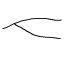
\includegraphics[width=0.4\textwidth]{fingerprints/minucje/rozwidlenie1.jpg}
                \caption*{Rozwidlenie pojedyncze}
            \end{figure}
        \column{0.25\textwidth}
            \begin{figure}[t]
			    \centering
                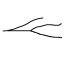
\includegraphics[width=0.4\textwidth]{fingerprints/minucje/rozwidlenie2.jpg}
                \caption*{Rozwidlenie podwójne}
            \end{figure}
    \end{columns}
    
    \begin{columns}
        \column{0.25\textwidth}
            \begin{figure}[t]
			    \centering
                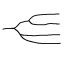
\includegraphics[width=0.4\textwidth]{fingerprints/minucje/rozwidlenie3.jpg}\\~\
                \caption*{Rozwidlenie potrójne}
            \end{figure}
		\column{0.25\textwidth}
		    \begin{figure}[t]
			    \centering
                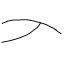
\includegraphics[width=0.4\textwidth]{fingerprints/minucje/zlaczenie1.jpg}\\~\
                \caption*{Złączenie pojedyncze}
            \end{figure}
        \column{0.25\textwidth}
            \begin{figure}[t]
                \centering
                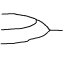
\includegraphics[width=0.4\textwidth]{fingerprints/minucje/zlaczenie2.jpg}\\~\
                \caption*{Złączenie podwójne}
            \end{figure}
        \column{0.25\textwidth}
            \begin{figure}[t]
			    \centering
                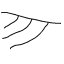
\includegraphics[width=0.4\textwidth]{fingerprints/minucje/zlaczenie3.jpg}\\~\
                \caption*{Złączenie potrójne}
            \end{figure}
    \end{columns}
\end{frame}

\begin{frame}{Minucje}
    \begin{columns}
        \column{0.25\textwidth}
            \begin{figure}[t]
			    \centering
                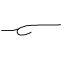
\includegraphics[width=0.4\textwidth]{fingerprints/minucje/haczyk.jpg}\\~\
                \caption*{Haczyk}
            \end{figure}
		\column{0.25\textwidth}
		    \begin{figure}[t]
			    \centering
                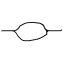
\includegraphics[width=0.4\textwidth]{fingerprints/minucje/oczko1.jpg}\\~\
                 \caption*{Oczko pojedyncze}
            \end{figure}
        \column{0.25\textwidth}
            \begin{figure}[t]
			    \centering
                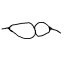
\includegraphics[width=0.4\textwidth]{fingerprints/minucje/oczko2.jpg}\\~\
                \caption*{Oczko podwójne}
            \end{figure}
        \column{0.25\textwidth}
            \begin{figure}[t]
			    \centering
                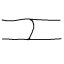
\includegraphics[width=0.4\textwidth]{fingerprints/minucje/mostek1.jpg}\\~\
                \caption*{Mostek pojedynczy}
            \end{figure}
    \end{columns}
    
    \begin{columns}
        \column{0.25\textwidth}
            \begin{figure}[t]
			    \centering
                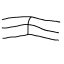
\includegraphics[width=0.4\textwidth]{fingerprints/minucje/mostek2.jpg}\\~\
                 \caption*{Mostek podwójny}
            \end{figure}
		\column{0.25\textwidth}
		    \begin{figure}[t]
			    \centering
                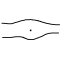
\includegraphics[width=0.4\textwidth]{fingerprints/minucje/punkt.jpg}\\~\
                \caption*{Punkt}
            \end{figure}
        \column{0.25\textwidth}
            \begin{figure}[t]
			    \centering
                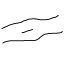
\includegraphics[width=0.4\textwidth]{fingerprints/minucje/odcinek.jpg}\\~\
                \caption*{Odcinek}
            \end{figure}
        \column{0.25\textwidth}
            \begin{figure}[t]
			    \centering
                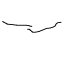
\includegraphics[width=0.4\textwidth]{fingerprints/minucje/styk_boczny.jpg}\\~\
                \caption*{Styk boczny}
            \end{figure}
    \end{columns}
\end{frame}

\begin{frame}{Minucje}
    \begin{columns}
        \column{0.33\textwidth}
            \begin{figure}[t]
    			\centering
                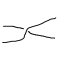
\includegraphics[width=0.3\textwidth]{fingerprints/minucje/linia_przech.jpg}\\~\
                \caption*{Linia przechodząca}
            \end{figure}
		\column{0.33\textwidth}
		    \begin{figure}[t]
        		\centering
                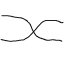
\includegraphics[width=0.3\textwidth]{fingerprints/minucje/skrzyzowanie.jpg}\\~\
                \caption*{Skrzyżowanie}
            \end{figure}
        \column{0.33\textwidth}
            \begin{figure}[t]
    			\centering
                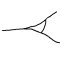
\includegraphics[width=0.3\textwidth]{fingerprints/minucje/trojnog.jpg}\\~\
                \caption*{Trójnóg}
            \end{figure}
    \end{columns}
    
    \begin{columns}
        \column{0.33\textwidth}
            \begin{figure}[t]
			    \centering
                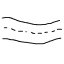
\includegraphics[width=0.3\textwidth]{fingerprints/minucje/linia_szczatkowa.jpg}\\~\
                \caption*{Linia szczątkowa}
            \end{figure}
        \column{0.33\textwidth}
            \begin{figure}[t]
			    \centering
                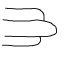
\includegraphics[width=0.3\textwidth]{fingerprints/minucje/minucja_m.jpg}\\~\
                \caption*{Minucja typu M}
            \end{figure}
    \end{columns}
\end{frame}

\begin{frame}{Minucje}
    \centering
    Przykładowe minucje na odcisku palca \\~\
    \smallskip
    \begin{figure}[t]
        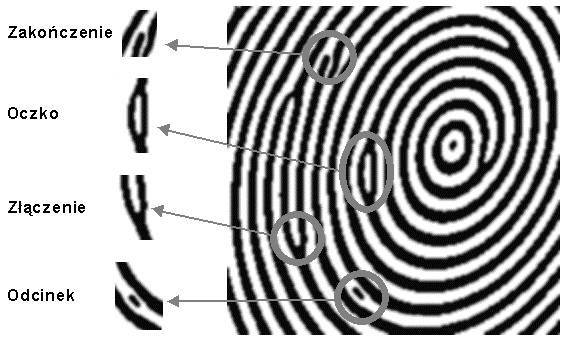
\includegraphics[width=0.53\textwidth]{fingerprints/minucje/minucje.jpg}
    \end{figure}
\end{frame}

\section{Algorytmy analizy}

\begin{frame}
    \centering
    \huge
    Algorytmy analizy
\end{frame}

\begin{frame}{Metoda oparta na analizie minucji}
    \begin{itemize}
    	\item Metoda polega na analizie poszczególnych minucji i porównaniu ich z wzorcem
        \item Wzorzec to najczęściej wektor zawierający punkty i względną odległość od innych
        \item Poszczególny punkt składa się z (względnej) pozycji, typu oraz kierunku
        \item Najczęściej stosowana metoda
	\end{itemize}
\end{frame}

\begin{frame}{Metoda oparta na analizie minucji}
    \begin{figure}[t]
        \centering
        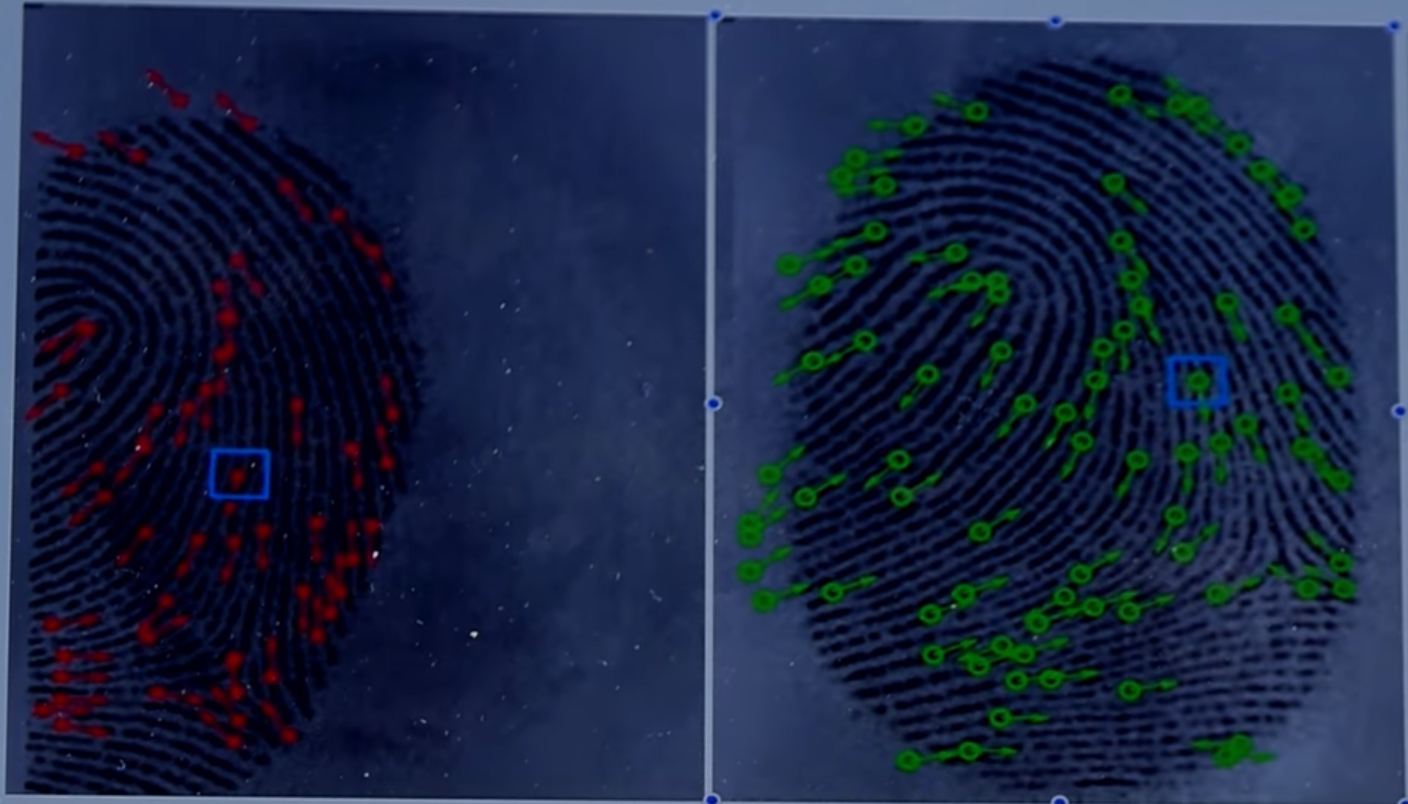
\includegraphics[width=0.85\linewidth]{algorithms/minuncje.png}
        \caption{Wizualizacja punktów minucji naniesiona na obrazy wejściowe}
    \end{figure}
\end{frame}

\begin{frame}{Metoda oparta na analizie minucji}
    \begin{figure}[t]
        \centering
        \includegraphics[width=0.4\linewidth]{algorithms/minuncje1.png}
        \caption{Naniesione na siebie obrazy z poprzedniego slajdu}
    \end{figure}
\end{frame}

\begin{frame}{Metoda oparta na porównaniu obrazów}
    \begin{enumerate}
        \item Wybór wzorcowych minucji
        \item Analiza zgodności minucji w badanym obrazie
        \item Podjęcie decyzji na podstawie uzyskanych wyników
    \end{enumerate}
\end{frame}

\begin{frame}{Metoda oparta na porównaniu obrazów}
    \begin{figure}[t]
        \centering
        \includegraphics[width=0.65\linewidth]{algorithms/Correlation_testing.png}
        \caption{Zasada działania algorytmu}
    \end{figure}
\end{frame}

\begin{frame}{Metoda oparta na porównaniu obrazów}
    \begin{figure}[t]
        \centering
        \includegraphics[width=0.65\linewidth]{algorithms/Corelation_distance.png}
        \caption{Podejmowanie decyzji}
    \end{figure}
\end{frame}

\begin{frame}{Metoda oparta na porównaniu obrazów}
    Zalety:
    \begin{itemize}
        \item Przydatna w przypadku, gdy dostarczane dane (obrazy) są niskiej jakości - trudna detekcja minucji
        \item Błędnie wykryte minucje nie wpływają na wynik analizy
        \item Wyodrębnione zostają pary wycinków obrazów co wpływa na wydajność porównania
    \end{itemize}
\end{frame}

\begin{frame}{Metoda oparta na porównaniu obrazów}
    Wady:
    \begin{itemize}
        \item Wymaga stosunkowo wysokiej mocy obliczeniowej
        \item Radzi sobie z rotacjami do 10\degree
        \item Z powodu powolnej analizy jest mało przydatna w aplikacjach działających w czasie rzeczywistym
    \end{itemize}
\end{frame}

\begin{frame}{Metoda oparta o krawędzie}
    Ekstrakcja minucji w obrazach niskiej jakości jest zagadnieniem trudnym. Jako rozwiązanie tego problemu powstały metody dopasowywania oparte m.in. o lokalne kierunki krawędzi linii papilarnych i częstość występowania krawędzi.
\end{frame}

\begin{frame}{Metoda oparta o krawędzie}
    Obraz linii papilarnych jest podzielony na wiele małych komórek. Lokalizacja linii w każdej komórce jest opisana parametrami pewnej fali sinusoidalnej. \\~\
    \begin{figure}[t]
        \centering
        \includegraphics[width=0.53\textwidth]{algorithms/krawedzie.png}
    \end{figure}
\end{frame}

\begin{frame}{Metoda oparta o krawędzie}
    Ta metoda może operować na obrazach gorszej jakości, dla których poprawne rozpoznanie minucji może nie być możliwe. Z drugiej jednak strony struktura linii papilarnych może być mniej unikalna niż struktura minucji. Metody te nie są powszechnie wykorzystywane z uwagi na coraz lepszą jakość obrazu dostarczanego przez czytniki.
\end{frame}

\section{Zakończenie}

\begin{frame}[allowframebreaks]
    \frametitle{Bibliografia}
    \begin{thebibliography}{6}
        \tiny
        \bibitem{Smithsonian}
        \url{https://www.smithsonianmag.com/smart-news/ancient-fingerprints-show-both-women-and-men-made-pottery-chaco-canyon-180972350/}
        \bibitem{FingerprintHistory}
        \url{https://www.onin.com/fp/fphistory.html}
        \bibitem{FingerprintHistoryPolish}
        \url{https://www.spyshop.pl/blog/historia-niezmazywalnej-pieczeci-czyli-jak-daktyloskopia-rozwijala-skrzydla/}
        \bibitem{}
        \url{https://kcir.pwr.edu.pl/~witold/aiarr/2009_projekty/odciski/}
        \bibitem{}
        \url{https://www.360biometrics.com/faq/fingerprint_scanners.php}
        \bibitem{}
        \url{http://ics.p.lodz.pl/~stolarek/_media/pl:research:stolarek_praca_magisterska.pdf}
        \bibitem{}
        \url{https://engineering.nyu.edu/news/so-you-think-you-can-secure-your-mobile-phone-fingerprint}
        \bibitem{}
        \url{https://www.slideshare.net/mahesamrin/correlation-based-fingerprint-recognition}
    \end{thebibliography}
\end{frame}

\begin{frame}
    \centering
    \begin{figure}[t]
        \centering
        \includegraphics[width=0.75\linewidth]{questions.png}
    \end{figure}
    \smallskip
    \Large
    Jakieś pytania?
\end{frame}

\begin{frame}
    \centering
    \huge
    Dziękujemy za uwagę
\end{frame}

\end{document}
